\section{UDSOnLIN}
\subsection{osi模型}

对USDonLIN而言,如图\ref{fig:usd_onlin}所示,各层使用的标准如下:
\begin{figure}[ht]
    \centering
    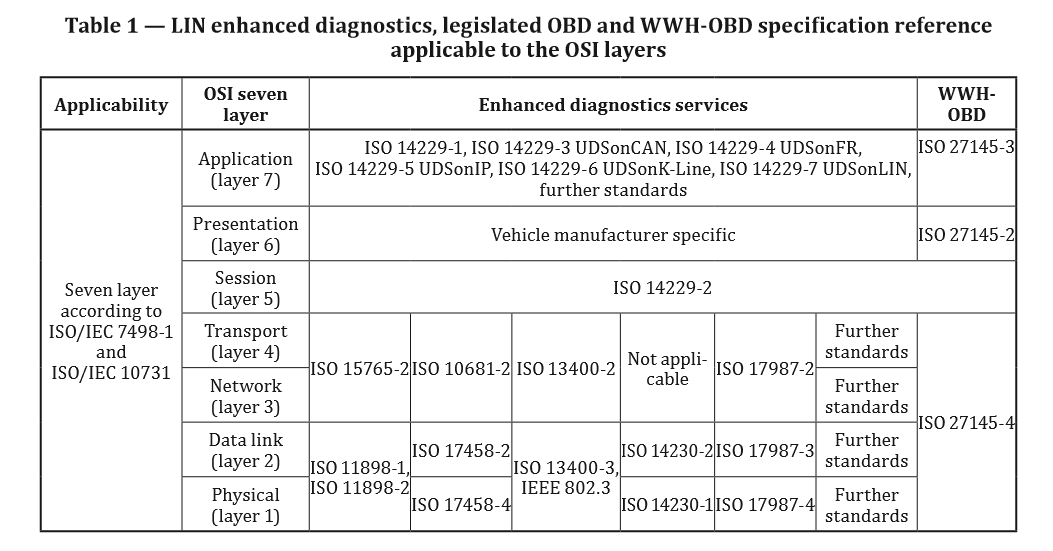
\includegraphics[scale=0.8]{./pic/osi_uds_onlin.png}
    \caption{osi uds on LIN}
    \label{fig:usd_onlin}
\end{figure}
对于LIN,物理层、数据链路层和网络层使用的标准为ISO 178974/3/2。

\subsection{符号和术语}

\begin{enumerate}
    \item AE address extension
    \item CF consecutive frame 连续帧
    \item DA destination address 
    \item FC flow control 
    \item FF first frame 
    \item ID identifier 
    \item Mtype message type 
    \item NAD node address 
    \item NCF node configuration file 
    \item P2 server response time 
    \item SA source address 
    \item SF single frame 
    \item SFID sub-function identifier 
    \item STmin separation time 
    \item TA target address 
    \item UART universal asynchronous receiver transmitter
\end{enumerate}